


\chapter{Performance Evaluation}  
This section presents the results of our models on the classification tasks and on the misinformation rebuttal task. The results show each model's precision, recall, f1 score, training time, and BERTScore.


\section{Health-Related Classification}
We present the results of the health classification process and compare them with the best overall model of the previous THS project \cite{8622504}. That work concluded
that their best model is an LSTM, with no attention, and a GRU layer.

\subsection{Precision}
\begin{table}[H]
	\centering
	\caption{Health Related Precision Result}
	\begin{tabular}{||c | c||} 
		\hline
		\textbf{Model} & \textbf{Result} \\ [0.5ex] 
		\hline
		BERT & 0.85  \\
		\hline
		LLaMa-2 & 0.94 \\ 
		\hline
		LSTM GRU NO ATTENTION & 0.83  \\
		\hline
		T5 (Causal) & 0.85 \\
		\hline
		T5 (Sequence) & 0.48 \\
		\hline
	\end{tabular}
	\label{table:HealthPrecision}
\end{table}

Table \ref{table:HealthPrecision} shows the result for the precision metric for the related classification. For clarity, we focus on this class because our project
goal is to detect health-related misinformation. The best-performing model here was the LLaMa-2 model, which has a precision of 94\%. Tied for second place
are BERT and T5 (Causal), with 85\% precision. Next is the THS model, with 83\% precision. Lastly, we have a T5 (Sequence) model with a relatively low
precision of 48\%.

\subsection{Recall}
\begin{table}[H]
	\centering
	\caption{Health Related Recall Result}
	\begin{tabular}{||c | c||} 
		\hline
		\textbf{Model} & \textbf{Result} \\ [0.5ex] 
		\hline
		BERT & 0.91  \\
		\hline
		LLaMa-2 & 0.84 \\ 
		\hline
		LSTM GRU NO ATTENTION & 0.89  \\
		\hline
		T5 (Causal) & 0.95 \\
		\hline
		T5 (Sequence) & 0.44 \\
		\hline
	\end{tabular}
	\label{table:HealthRecall}
\end{table}

Table \ref{table:HealthRecall} shows the result for the recall metric for the related classification. When comparing this metric with the THS investigation, there is a noticeable difference. Their results
show that only the LSTM layer, no attention, and a GRU layer model was the only one with a result over 80\%. In contrast, most of our models had a score of at least 80\%. Comparing this result
with the precision table (Table \ref{table:HealthPrecision}, our model did not score drastically lower. Here, our best model was T5 (Causal), with a performance of 95\% in recall. Next, we have
BERT with 91\%, followed by the THS model with 89\%. Then, the model with the highest precision, LLaMa-2, ended with 84\%. Lastly, we have again the T5 (Sequence) model with a 44\%,
lower than its precision.

\subsection{F1}
\begin{table}[H]
	\centering
	\caption{Health Related F1 Result}
	\begin{tabular}{||c | c||} 
		\hline
		\textbf{Model} & \textbf{Result} \\ [0.5ex] 
		\hline
		BERT & 0.88  \\
		\hline
		LLaMa-2 & 0.89 \\ 
		\hline
		LSTM GRU NO ATTENTION & 0.86  \\
		\hline
		T5 (Causal) & 0.90 \\
		\hline
		T5 (Sequence) & 0.46 \\
		\hline
	\end{tabular}
	\label{table:HealthF1}
\end{table}

Table \ref{table:HealthF1} shows the result for the F1 metric for the related classification. The F1 score is the balance between precision and recall. When we compare the results with the
THS model, most models have a higher F1 score. The results show that T5 (Causal) had 90\%, LLaMa-2 with 89\%, BERT ended with 88\%, and T5 (Sequence) scored a 46\%. In contrast,
the THS model had an 86\%, ending in second to last place.

\subsection{Training Time}

In Figure \ref{fig:HealthTime}, we present our model's training time. As mentioned earlier, we trained each model for 20 epochs with a batch size of 16. BERT trained faster than
any other model, which took 187 minutes. The T5 (Sequence) model took 1442 minutes, while the T5 (Causal) model finished in 1569 minutes. Lastly, LLaMa-2 took 5126 minutes to
train. Based on these results, we can infer that models with fewer parameters train faster. BERT trained 27.4x faster than LLaMa-2.

\begin{figure}[H]
	\begin{center}
		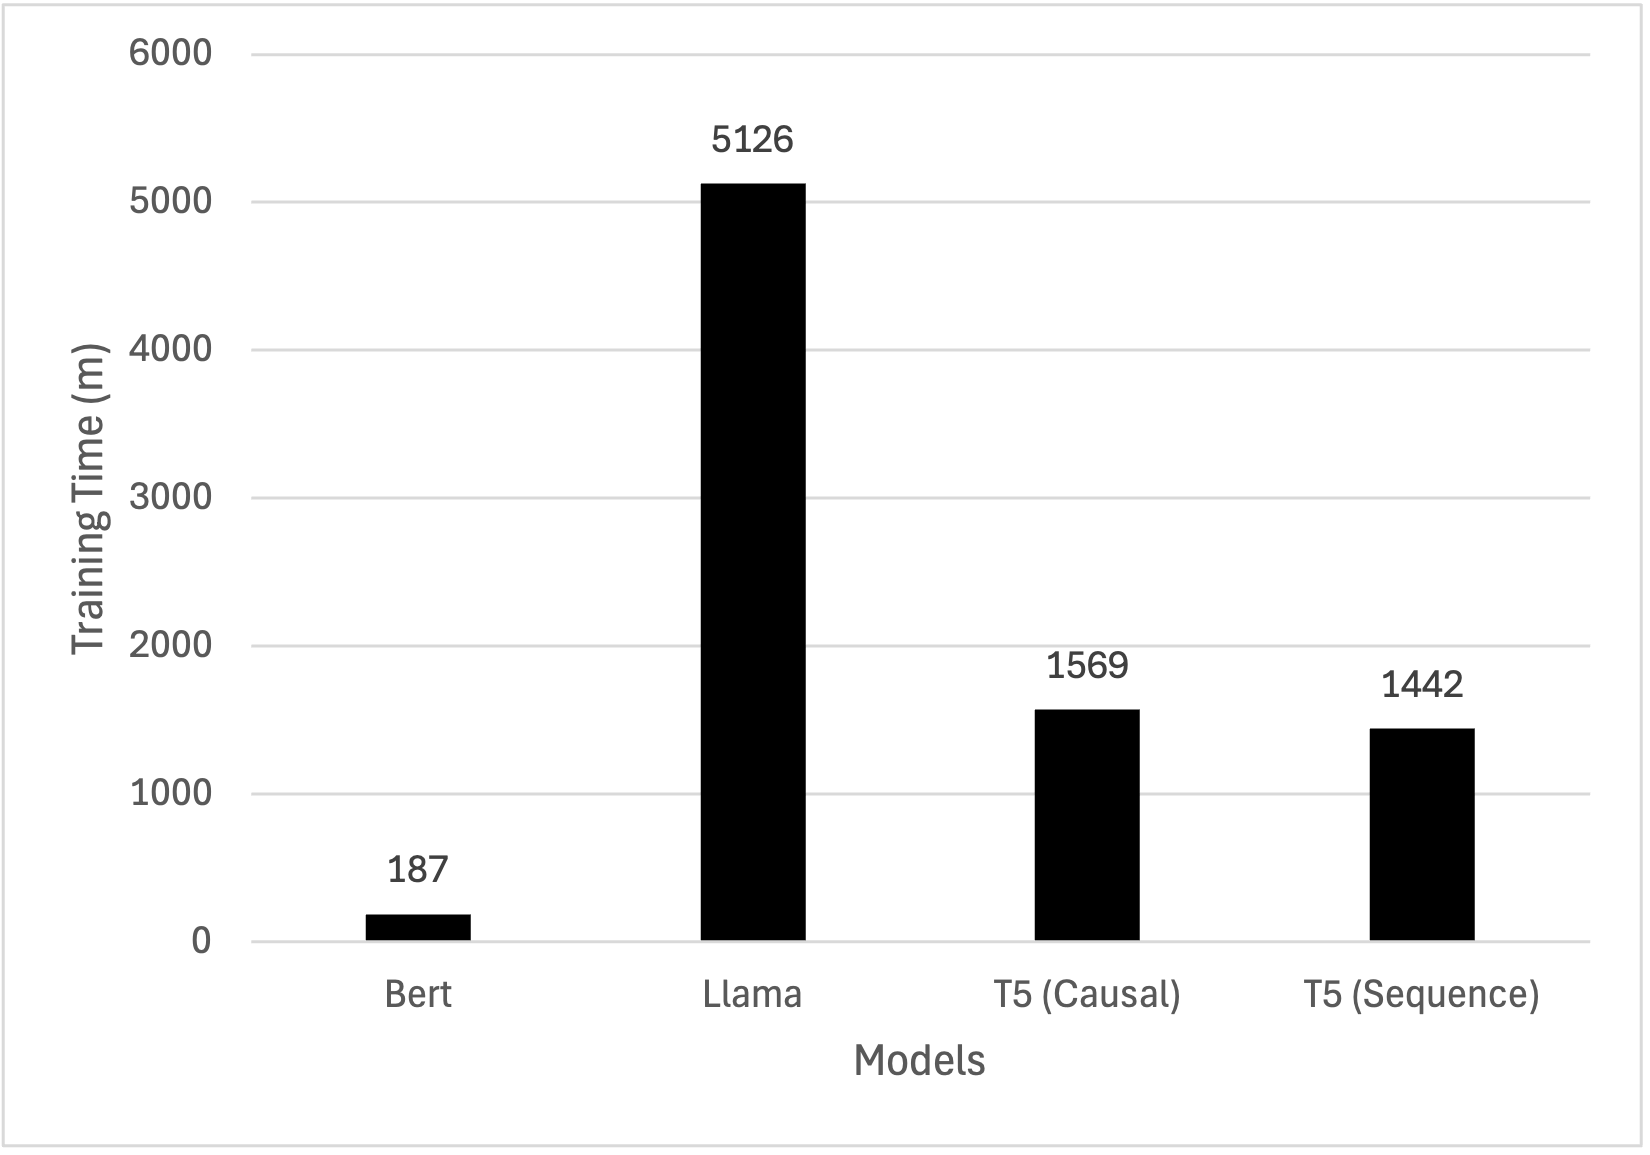
\includegraphics[width=1\textwidth]{images/Health_related_training_time.png} %specify width
	\end{center}
	\caption{Health-Related Models Training Time} %specify caption
	\label{fig:HealthTime}
\end{figure}


\section{Misinformation Classification}
In this section, we present the misinformation classification results. However, in this section, we did not compare with the THS model because they did not train a model to classify
misinformation.

\subsection{Precision}
\begin{table}[H]
	\centering
	\caption{Misinformation Precision Result}
	\begin{tabular}{||c | c||} 
		\hline
		\textbf{Model} & \textbf{Result} \\ [0.5ex] 
		\hline
		BERT & 0.90  \\
		\hline
		LLaMa-2 & 0.98 \\ 
		\hline
		T5 (Causal) & 0.99 \\
		\hline
		T5 (Sequence) & 0.99 \\
		\hline
	\end{tabular}
	\label{table:MisinformationPrecision}
\end{table}

Table \ref{table:MisinformationPrecision} shows the result for the precision metric for the misinformation classification. In this case, we focus on the misinformation
class because it is our project goal. Our best-performing models here were both T5 models, which have a precision of 99\%. The next model with the highest precision
was LLaMa-2, with a score of 98\% precision. The lowest-performing model was BERT, which resulted in 90\% precision. Nonetheless, all models had a score of at least 90\%.


\subsection{Recall}
\begin{table}[H]
	\centering
	\caption{Misinformation Recall Result}
	\begin{tabular}{||c | c||} 
		\hline
		\textbf{Model} & \textbf{Result} \\ [0.5ex] 
		\hline
		BERT & 0.94  \\
		\hline
		LLaMa-2 & 0.95 \\ 
		\hline
		T5 (Causal) & 0.92 \\
		\hline
		T5 (Sequence) & 0.85 \\
		\hline
	\end{tabular}
	\label{table:MisinformationRecall}
\end{table}

Table \ref{table:MisinformationRecall} shows the recall metric's results for the misinformation classification. When we compare these results with the precision table 
(Table \ref{table:MisinformationPrecision}), our model maintains a similar score. Here, the model with the best results was LLaMa-2, with a performance of 95\%.
Next, we have BERT with 94\% and T5 (Causal) with a 92\% recall. Finally, T5 (Sequence) ended with 85\% in the recall.


\subsection{F1}
\begin{table}[H]
	\centering
	\caption{Misinformation F1 Result}
	\begin{tabular}{||c | c||} 
		\hline
		\textbf{Model} & \textbf{Result} \\ [0.5ex] 
		\hline
		BERT & 0.92  \\
		\hline
		LLaMa-2 & 0.97 \\ 
		\hline
		T5 (Causal) & 0.96 \\
		\hline
		T5 (Sequence) & 0.92 \\
		\hline
	\end{tabular}
	\label{table:MisinformationF1}
\end{table}


Table \ref{table:MisinformationF1}  shows the result for the F1 metric for the misinformation classification. This result balances precision and recall. The results show that the model
with the best F1 was LLaMa-2 with a 97\%. Next is T5 (Causal) with a 96\% F1, and tied to last, we have BERT and T5 (Sequence) with 92\%. All models had an optimal F1 score over 90\%.


\subsection{Training Time}

In Figure \ref{fig:MisinformationTime}, we present the training time for the misinformation models. We trained the models using the same parameters as in the Health-Related classification.
When we compare these results with the Health-Related (Figure \ref{fig:HealthTime}), the average training time was less. A possible reason is that we used less data for the training. The
only exception was BERT, which took 351 minutes to train. Next is T5 (Causal) with 371 minutes and T5 (Sequence) with 1274 minutes. Finally, LLaMa-2 took 2840 minutes to train. A noticeable difference was T5 (Causal), which trained 4.23x faster for this dataset compared to the health-related dataset. Nonetheless, BERT finished the fastest, being 8.10x faster than LLaMa-2.


\begin{figure}[H]
	\begin{center}
		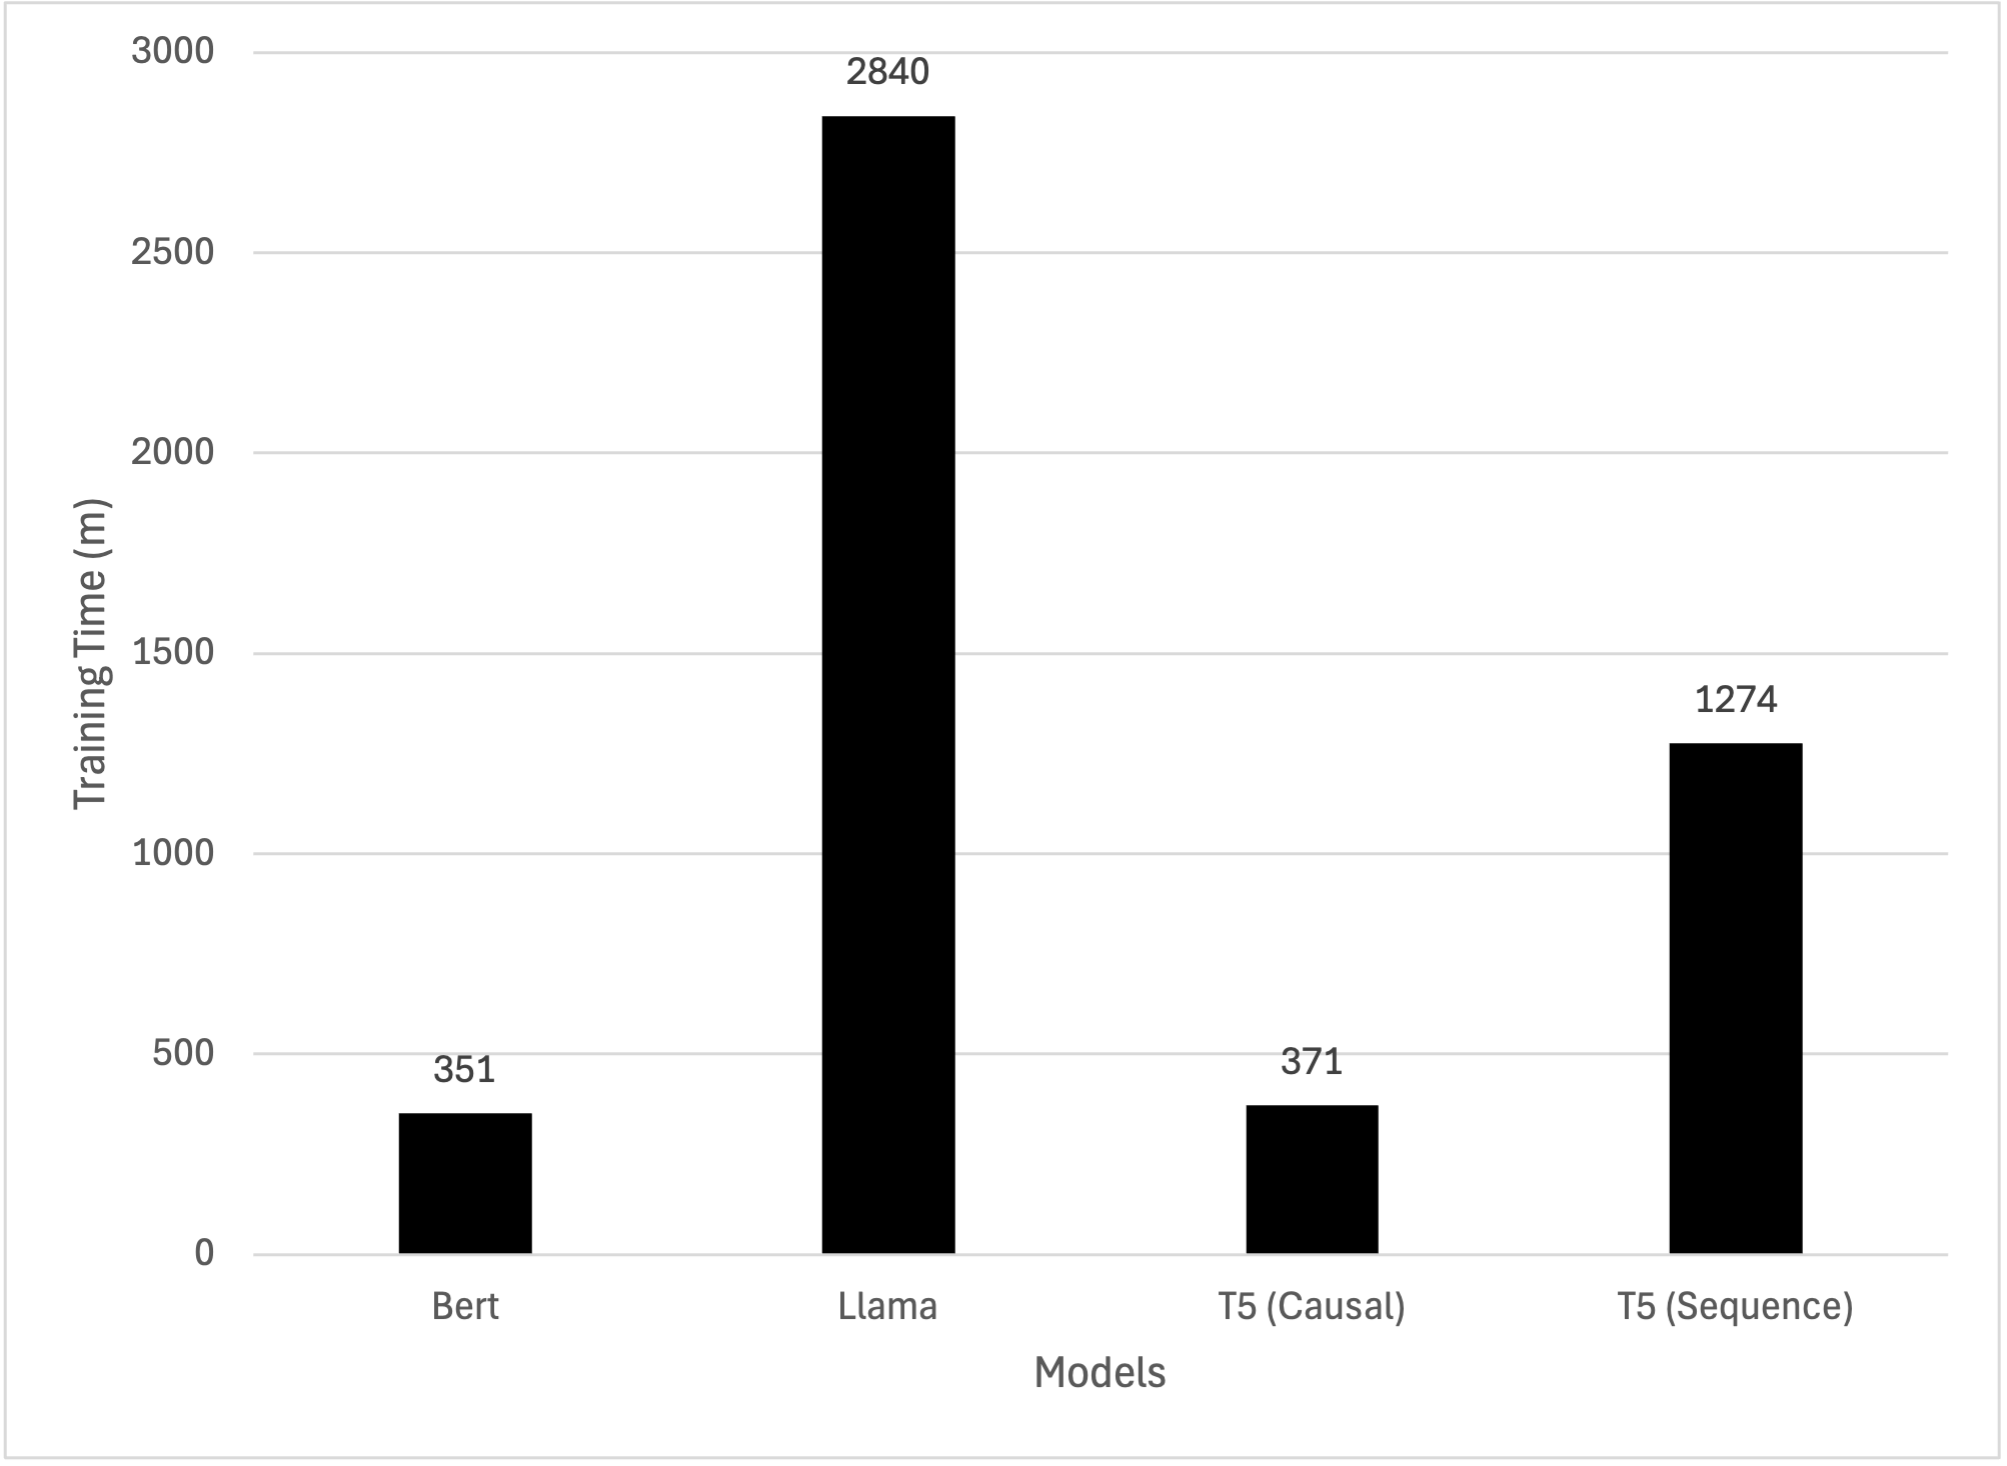
\includegraphics[width=1\textwidth]{images/Misinformation_training_time.png} %specify width
	\end{center}
	\caption{Misinformation Models Training Time} %specify caption
	\label{fig:MisinformationTime}
\end{figure}


\section{BERTScore}

Our model BERTScores'  F1 is shown in Table \ref{table:BERTScore}. We calculate these values by taking the average score of the 71 texts classified as health-related and misinformation. The table shows that both models, had a 82\% F1 score. That means that the generated output are closely related but not exactly the same. 

\begin{table}[H]
	\centering
	\caption{BERTScore F1 Results}
	\begin{tabular}{||c | c||} 
		\hline
		\textbf{Model} & \textbf{Result} \\ [0.5ex] 
		\hline
		LLaMa-3.1 & 82\%  \\
		\hline
		GPT-3.5-turbo & 82\% \\ 		
		\hline
		\end{tabular}
	\label{table:BERTScore}
\end{table}



\section{Discussion}

The results present that most LLMs outperformed the THS model. We applied preprocessing techniques such as replacing links, mentions, and hashtags with special tokens. The training
parameters for all models were 20 epochs, batch size of 16, 8bit initialization, and adamw\_8bit optimizer. Additionally, the LoRA hyperparameters were 16 for the rank, an alpha of 32, a dropout
of 0.05, and a bias for all parameters. The score metrics we used for the model evaluation were precision, recall, and F1. In our case, we want to focus on F1. That metric helps us reduce false
negative results but not overclassify false positives.

Our model with the best result for the health-related classification (Table \ref{table:HealthF1}) was T5 (Causal), with a 90\% F1 score, while the THS model had 86\%. However, the trade-off
for this model is that the training is computationally expensive. The reason is that labels in T5 (Causal) are text instead of numbers. Those texts must be embedded, which requires more
processing power. Also, that model cannot have class weights because of the structure of the embedding. Additionally, the training time  (Figure \ref{fig:HealthTime}) for T5 is more extensive
when compared to BERT, 8.4x. Now, BERT had a slightly lower result with 88\%. Nonetheless, when we factor in the training time and processing power, this model is more efficient.

The model with the highest F1 score for the misinformation classification (Table \ref{table:MisinformationF1}) was LLaMa-2, followed by T5 (Causal), 97\% and 96\%, respectively. These two models
have desirable results for this classification task. However, both require high computational power, and LLaMa-2 has an extensive training time (Figure \ref{fig:MisinformationTime}) compared to BERT,
8.09x more. It is important to notice that in both scenarios, LlaMa-2 and T5 (Causal) outperform the other models by a slight margin. These models contain a Decoder element, which can help them
generate and understand text appropriately.

For the BERTScore, we see that both models had an identical performance (Table \ref{table:BERTScore}). A possible reason is that the RAG process gives sufficient context to generate a coherent response. However, both models
have their trade-offs. To use GPT-3.5-turbo, we must pay OpenAI to request their API. On the other hand, LLaMa-3.1 ran with Ollama locally, and we need sufficient memory to execute the model. The
use case for each one depends on the user's hardware.

This project focuses on social media posts, and we know that there are frequent changes in how users interact. Additionally, when new diseases are found or named, we must retrain most
models to add these words to their vocabulary. Retraining can be costly if the model has many parameters and requires extensive training. Thus, we can say that BERT had overall results
that can help combat health misinformation on social media. That model had an F1 score of 88\% in health and 92\% in misinformation classification. Finally, that model took less overall time
to train and used the least amount of RAM.










